\documentclass[10pt]{article}

%si colocas esto se ve en times new roman, pero compilas es con xelatex
%\usepackage{fontspec}
%\setmainfont{Times New Roman}

\usepackage{tocbibind}

\usepackage[a4paper]{geometry}
\geometry{top=2.54cm, bottom=2.54cm, left=2.54cm, right=2.54cm}
\usepackage[spanish]{babel}

\usepackage{float}
\usepackage{graphicx} % graficos
\graphicspath{ {./images/} }
\usepackage{setspace}%interlineado agrega:
\usepackage{listings}
\usepackage{xcolor}
\usepackage{fancyvrb}
\definecolor{codegreen}{rgb}{0,0.6,0}
\definecolor{codegray}{rgb}{0.5,0.5,0.5}
\definecolor{codepurple}{rgb}{0.58,0,0.82}
\definecolor{backcolour}{rgb}{0.95,0.95,0.92}

\lstdefinestyle{mystyle}{
    backgroundcolor=\color{backcolour},
    commentstyle=\color{codegreen},
    keywordstyle=\color{magenta},
    numberstyle=\tiny\color{codegray},
    stringstyle=\color{codepurple},
    basicstyle=\ttfamily\footnotesize,
    breakatwhitespace=false,
    breaklines=true,
    captionpos=b,
    keepspaces=true,
    numbers=left,
    numbersep=5pt,
    showspaces=false,
    showstringspaces=false,
    showtabs=false,
    tabsize=2
}

\lstset{style=mystyle}
% \doublespacing \onehalfspace \singlespace \spacing{x}
\spacing{1.5}
\pagestyle{headings}

\usepackage[backend=biber, autocite=inline, labeldateparts=true, maxcitenames=1,style = apa]{biblatex}
\bibliography{referencias}

\usepackage{csquotes}
\usepackage[bookmarks = true, colorlinks=true, linkcolor = black, citecolor = black, menucolor = black, urlcolor = black]{hyperref}

\newcommand{\comillas}[1]{``#1"}

\begin{document}
\renewcommand{\listtablename}{Índice de Tablas}
\pagenumbering{roman}

	\setcounter{page}{0}
\begin{titlepage}

\begin{table}[t]
\centering
\begin{tabular}{ p{3cm} p{8.5cm} p{3cm} }
	\begin{flushleft}
\includegraphics[width=2.4cm]{logo_poli.png}\end{flushleft} &



	\begin{center}
	República Bolivariana de Venezuela\\
	Universidad Nacional Experimental Politécnica “Antonio José de Sucre”\\
	Vice Rectorado Barquisimeto \\
	Departamento de Ingeniería Electrónica\\  

%***************************************************
%************** aqui va el titulo ******************
%***************************************************

	\vspace*{65mm}
	\begin{LARGE}
		Practica 3\\ laboratorio de diseño de sistemas de computación
	\end{LARGE}

	\end{center}


	& \begin{flushright}
\includegraphics[width=1.7cm]{logo_electronica.jpg} \end{flushright}
\end{tabular}


	\vspace*{3mm}

	\parbox[c]{12cm}{
	\begin{center}
		\begin{small}
			
		\end{small}
	
	\end{center}
	}

	
	
	\vspace*{45mm}



\begin{flushright}
Integrantes:\\


Gerardo Alfonzo Campos Fonseca\\ 
V. 27085179\\
José Andrés Cortez Teran\\
V. 26540824\\

\vspace*{2mm}


\end{flushright}
\vspace*{5mm}

\begin{center}Barquisimeto, Julio del 2021\end{center}
\end{table}
\end{titlepage}



	\newpage
	\tableofcontents
	\newpage
	\listoffigures
	%\newpage
	%\listoftables

    %\newpage
    \pagenumbering{arabic}
	%\documentclass[10pt]{article}

\section*{Programa lectura.asm}

El código del programa se encuentra en un único archivo llamado \textbf{lectura.asm}.
Este programa funciona mediante una aplicación de consola usando la api de 32
bits de Windows. Para la lectura del archivo se usan las funciones
CreateFile en modo lectura, GetFileSize y ReadFile el tamaño. GetFileSize
se utiliza para crear un bloque de memoria lo suficientemente grande
para almacenar el archivo en memoria, mas el nuevo registro. Para escribir
el archivo una vez modificado se utilizan lstrlen para poder saber la cantidad
de bytes a escribir y finalmente se usa WriteFile.


\lstinputlisting[language={[x86masm]Assembler}]{practica5/consola/lectura.asm}

\section*{Funcionamiento del programa}

\begin{figure}[H]
  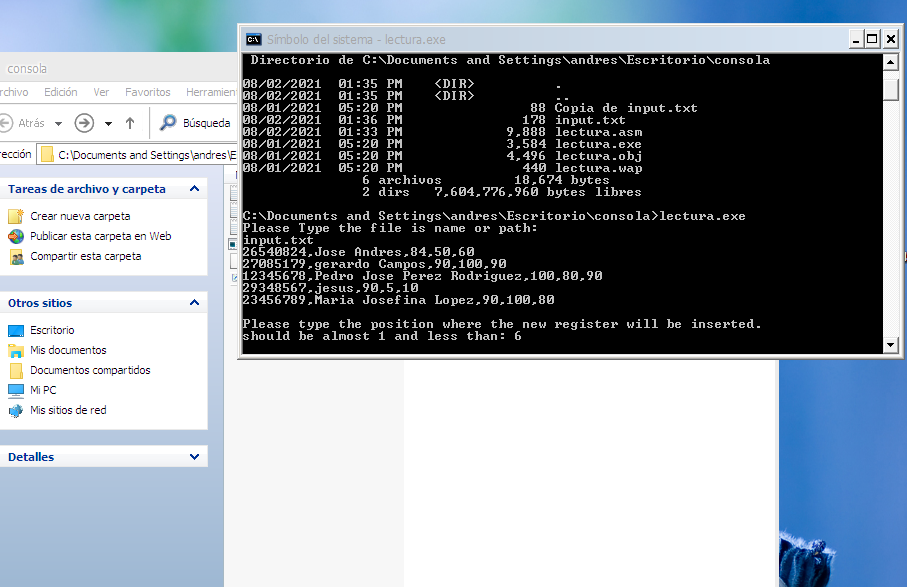
\includegraphics[width=\linewidth]{practica5/img/fig1}
    \caption{Abriendo el archivo}
\end{figure}

\begin{figure}[H]
  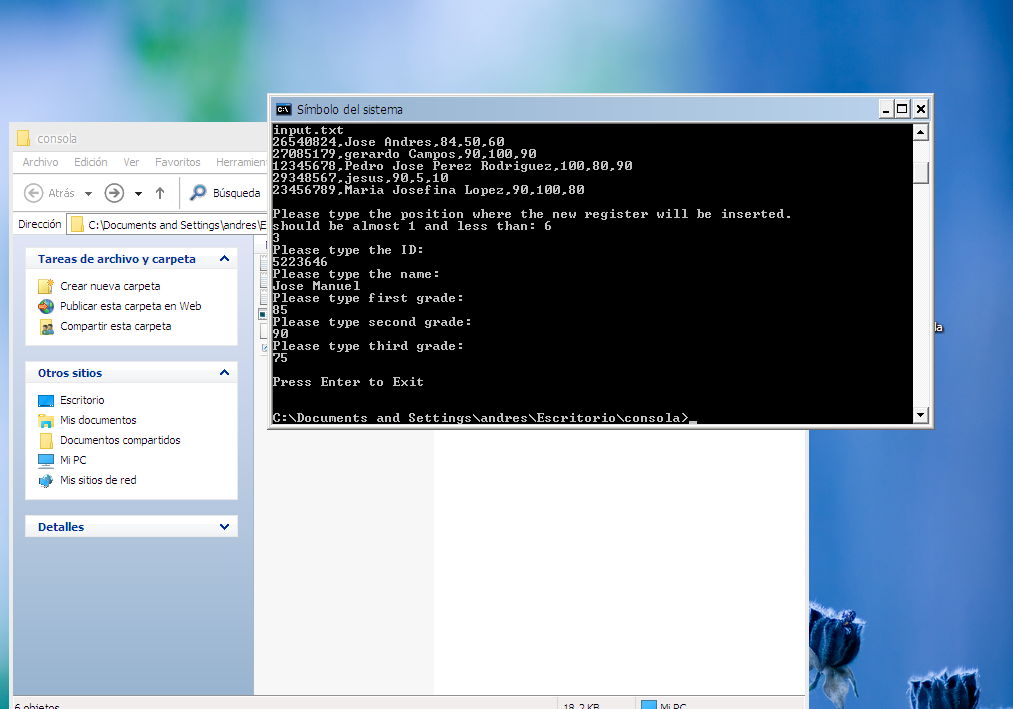
\includegraphics[width=\linewidth]{practica5/img/fig2}
    \caption{Agregando un nuevo registro}
\end{figure}

\begin{figure}[H]
  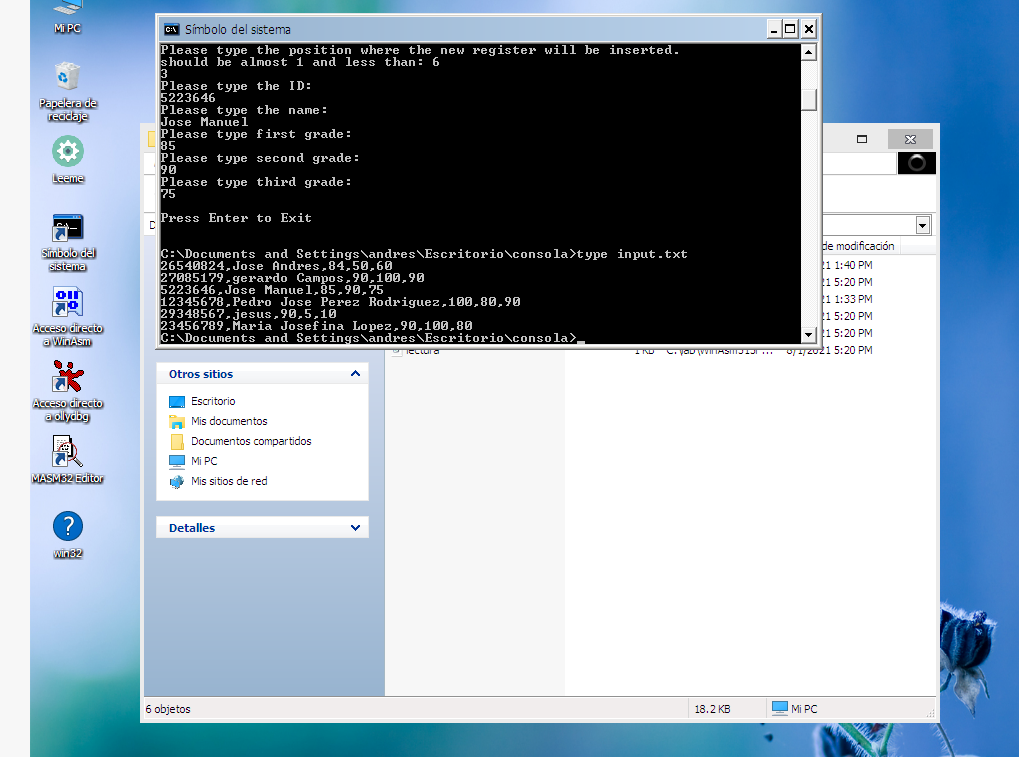
\includegraphics[width=\linewidth]{practica5/img/fig3}
    \caption{Mostrando en pantalla el archivo resultante}
\end{figure}

	\nocite{*}
	\printbibliography[title={\centering{Referencias Bibliográficas}}]

\end{document}
